\subsection{Planes de Trabajo del Proyecto}

Los planes de trabajo describen cómo se ejecutarán las principales actividades del proyecto durante su desarrollo. Esta sección define la descomposición de tareas, la calendarización, la asignación de recursos y la distribución del esfuerzo, estableciendo responsables, herramientas y momentos de ejecución para cada actividad relevante del proyecto.

\subsubsection{Descomposición de Actividades}

La estructura de descomposición de trabajo (WBS) del proyecto se construyó tomando como referencia las seis fases del enfoque Design Science Research (DSR) definido para el desarrollo del framework. Cada fase agrupa actividades técnicas, organizacionales y de validación asociadas a los principales entregables del proyecto.

Dado el carácter iterativo de la Fase 4 —correspondiente al desarrollo del artefacto— se presenta el detalle completo de una iteración representativa, incluyendo actividades de implementación, pruebas y validación incremental de los componentes del SDK. La gestión del proyecto se considera transversal a todas las fases y contempla actividades permanentes de seguimiento, documentación y control del avance.

1. Kit Pagos Colombia

1.1 Gestión del proyecto (transversal)

\begin{itemize}
  \item 1.1.1 Elaboración y mantenimiento del SPMP
  \item 1.1.2 Seguimiento semanal del backlog
  \item 1.1.3 Reportes quincenales de progreso al director
  \item 1.1.4 Registro de actas de reunión y decisiones clave
\end{itemize}

1.2 Fase 1 – Identificación del problema

\begin{itemize}
  \item 1.2.1 Análisis de autenticación, respuestas y webhooks de Wompi
  \item 1.2.2 Análisis de autenticación, respuestas y webhooks de PayU
  \item 1.2.3 Análisis de autenticación, respuestas y webhooks de Mercado Pago
  \item 1.2.4 Análisis de autenticación, respuestas y webhooks de Kushki
  \item 1.2.5 Consolidación del mapa comparativo del ecosistema (Hito H1)
  \item 1.2.6 Repositorio de parámetros de prueba por pasarela (Hito H1)
\end{itemize}

1.3 Fase 2 – Definición de objetivos

\begin{itemize}
  \item 1.3.1 Documento de alcance formal (SRS inicial)
  \item 1.3.2 Criterios de evaluación formalizados
  \item 1.3.3 Definición y documentación de los proyectos prototípicos
\end{itemize}

1.4 Fase 3 – Diseño

\begin{itemize}
  \item 1.4.1 Modelo de dominio unificado (clases y relaciones)
  \item 1.4.2 Especificación de puertos de la arquitectura hexagonal
  \item 1.4.3 Especificación de adaptadores por pasarela
  \item 1.4.4 Diseño de la API de simulación (endpoints y escenarios)
  \item 1.4.5 Registro de ADRs para decisiones arquitectónicas clave (Hito H2)
\end{itemize}

1.5 Fase 4 – Desarrollo iterativo

\begin{itemize}
  \item 1.5.1 Iteración 1 – Núcleo del SDK
  \item 1.5.1.1 Implementación del modelo de dominio y contratos de puerto
  \item 1.5.1.2 Pruebas unitarias del núcleo (cobertura $\geq$ 80 \%)
  \item 1.5.1.3 Revisión técnica grupal del núcleo (Hito H3 parcial)
\end{itemize}

1.5.2 Iteración 2 – Adaptadores de pasarela

\begin{itemize}
  \item 1.5.2.1 Desarrollo del adaptador Wompi con pruebas de integración
  \item 1.5.2.2 Desarrollo del adaptador PayU con pruebas de integración
  \item 1.5.2.3 Desarrollo del adaptador Mercado Pago con pruebas de integración
  \item 1.5.2.4 Desarrollo del adaptador Kushki con pruebas de integración
  \item 1.5.2.5 Validación cruzada de los cuatro adaptadores (Hito H3 completo)
\end{itemize}

1.5.3 Iteración 3 – API de simulación y soporte de validación

\begin{itemize}
  \item 1.5.3.1 Implementación de escenarios de prueba para las pasarelas soportadas
  \item 1.5.3.2 Despliegue de la API en Railway o Render
  \item 1.5.3.3 Documentación centralizada de datos de prueba
  \item 1.5.3.4 Colección Postman versionada en el repositorio (Hito H4)
\end{itemize}

1.6 Fase 5 – Demostración y evaluación

\begin{itemize}
  \item 1.6.1 Construcción de prototipos con integración directa a APIs nativas
  \item 1.6.2 Construcción de prototipos utilizando el framework desarrollado
  \item 1.6.3 Cálculo de métricas WMC, CBO y RFC mediante ts-morph
  \item 1.6.4 Elaboración del informe comparativo (Hito H5)
\end{itemize}

1.7 Fase 6 – Comunicación

\begin{itemize}
  \item 1.7.1 Redacción y revisión del documento final de trabajo de grado
  \item 1.7.2 Publicación del repositorio público con README, ejemplos y TypeDoc
  \item 1.7.3 Entrega formal y presentación ante director y evaluadores (Hito H6)
\end{itemize}

\subsubsection{Calendarización}

\begin{figure}[H]
  \centering
  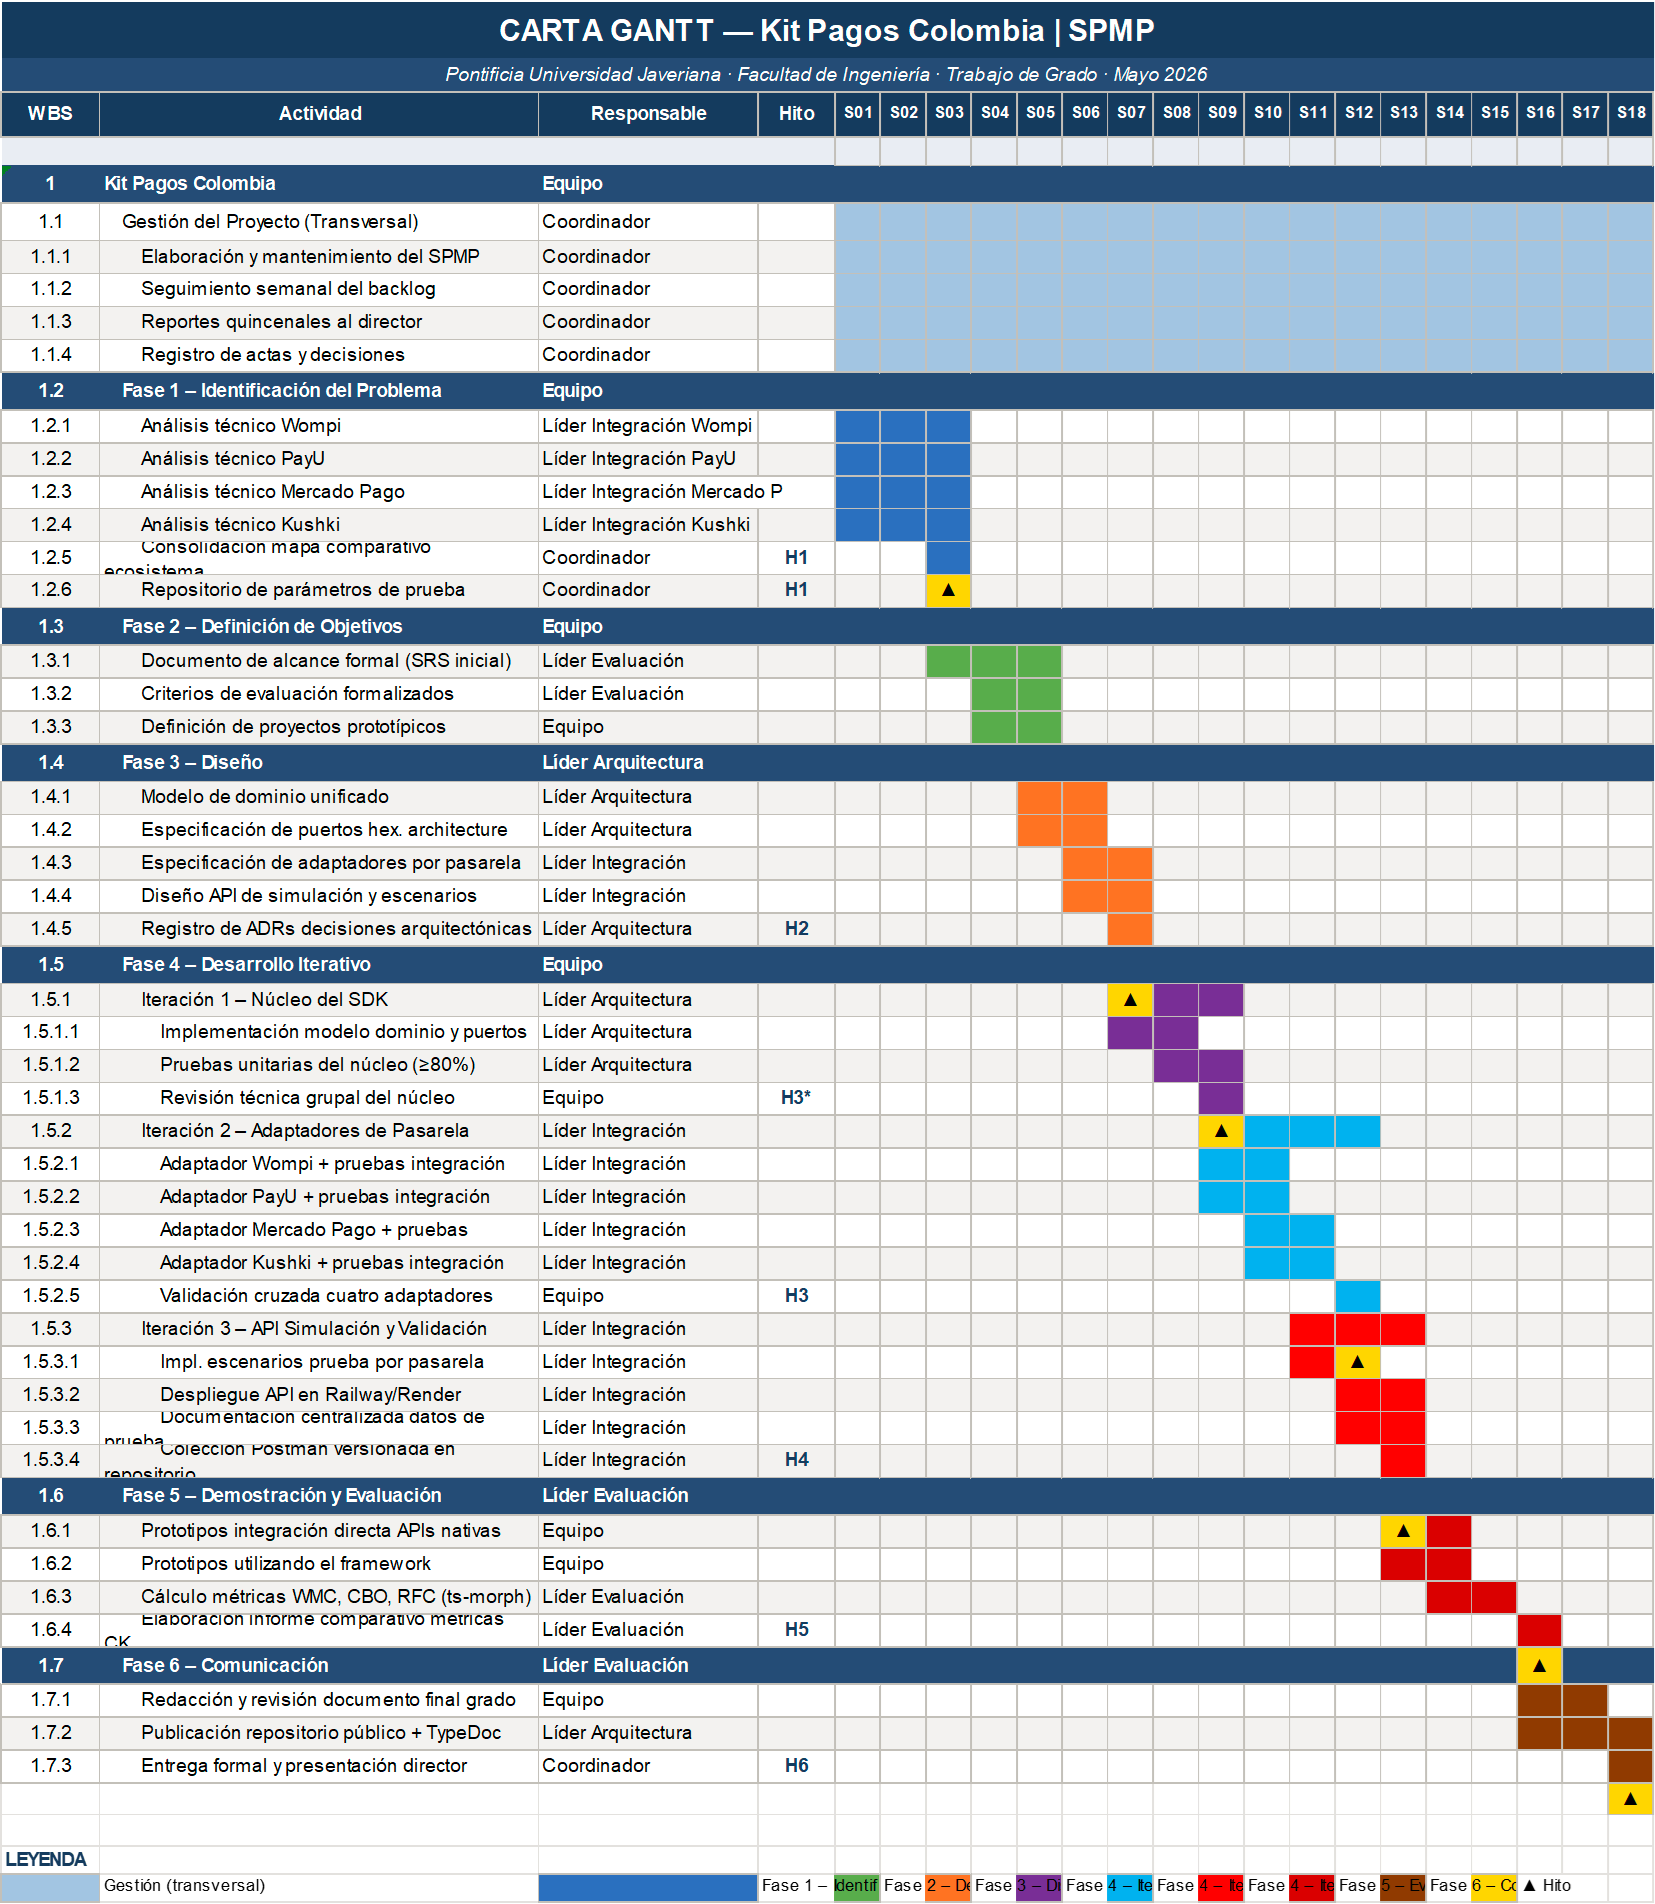
\includegraphics[width=\textwidth]{figuras/03-carta-gantt}
  \caption{Carta Gantt}
  \label{fig:carta-gantt}
\end{figure}

\begin{figure}[H]
  \centering
  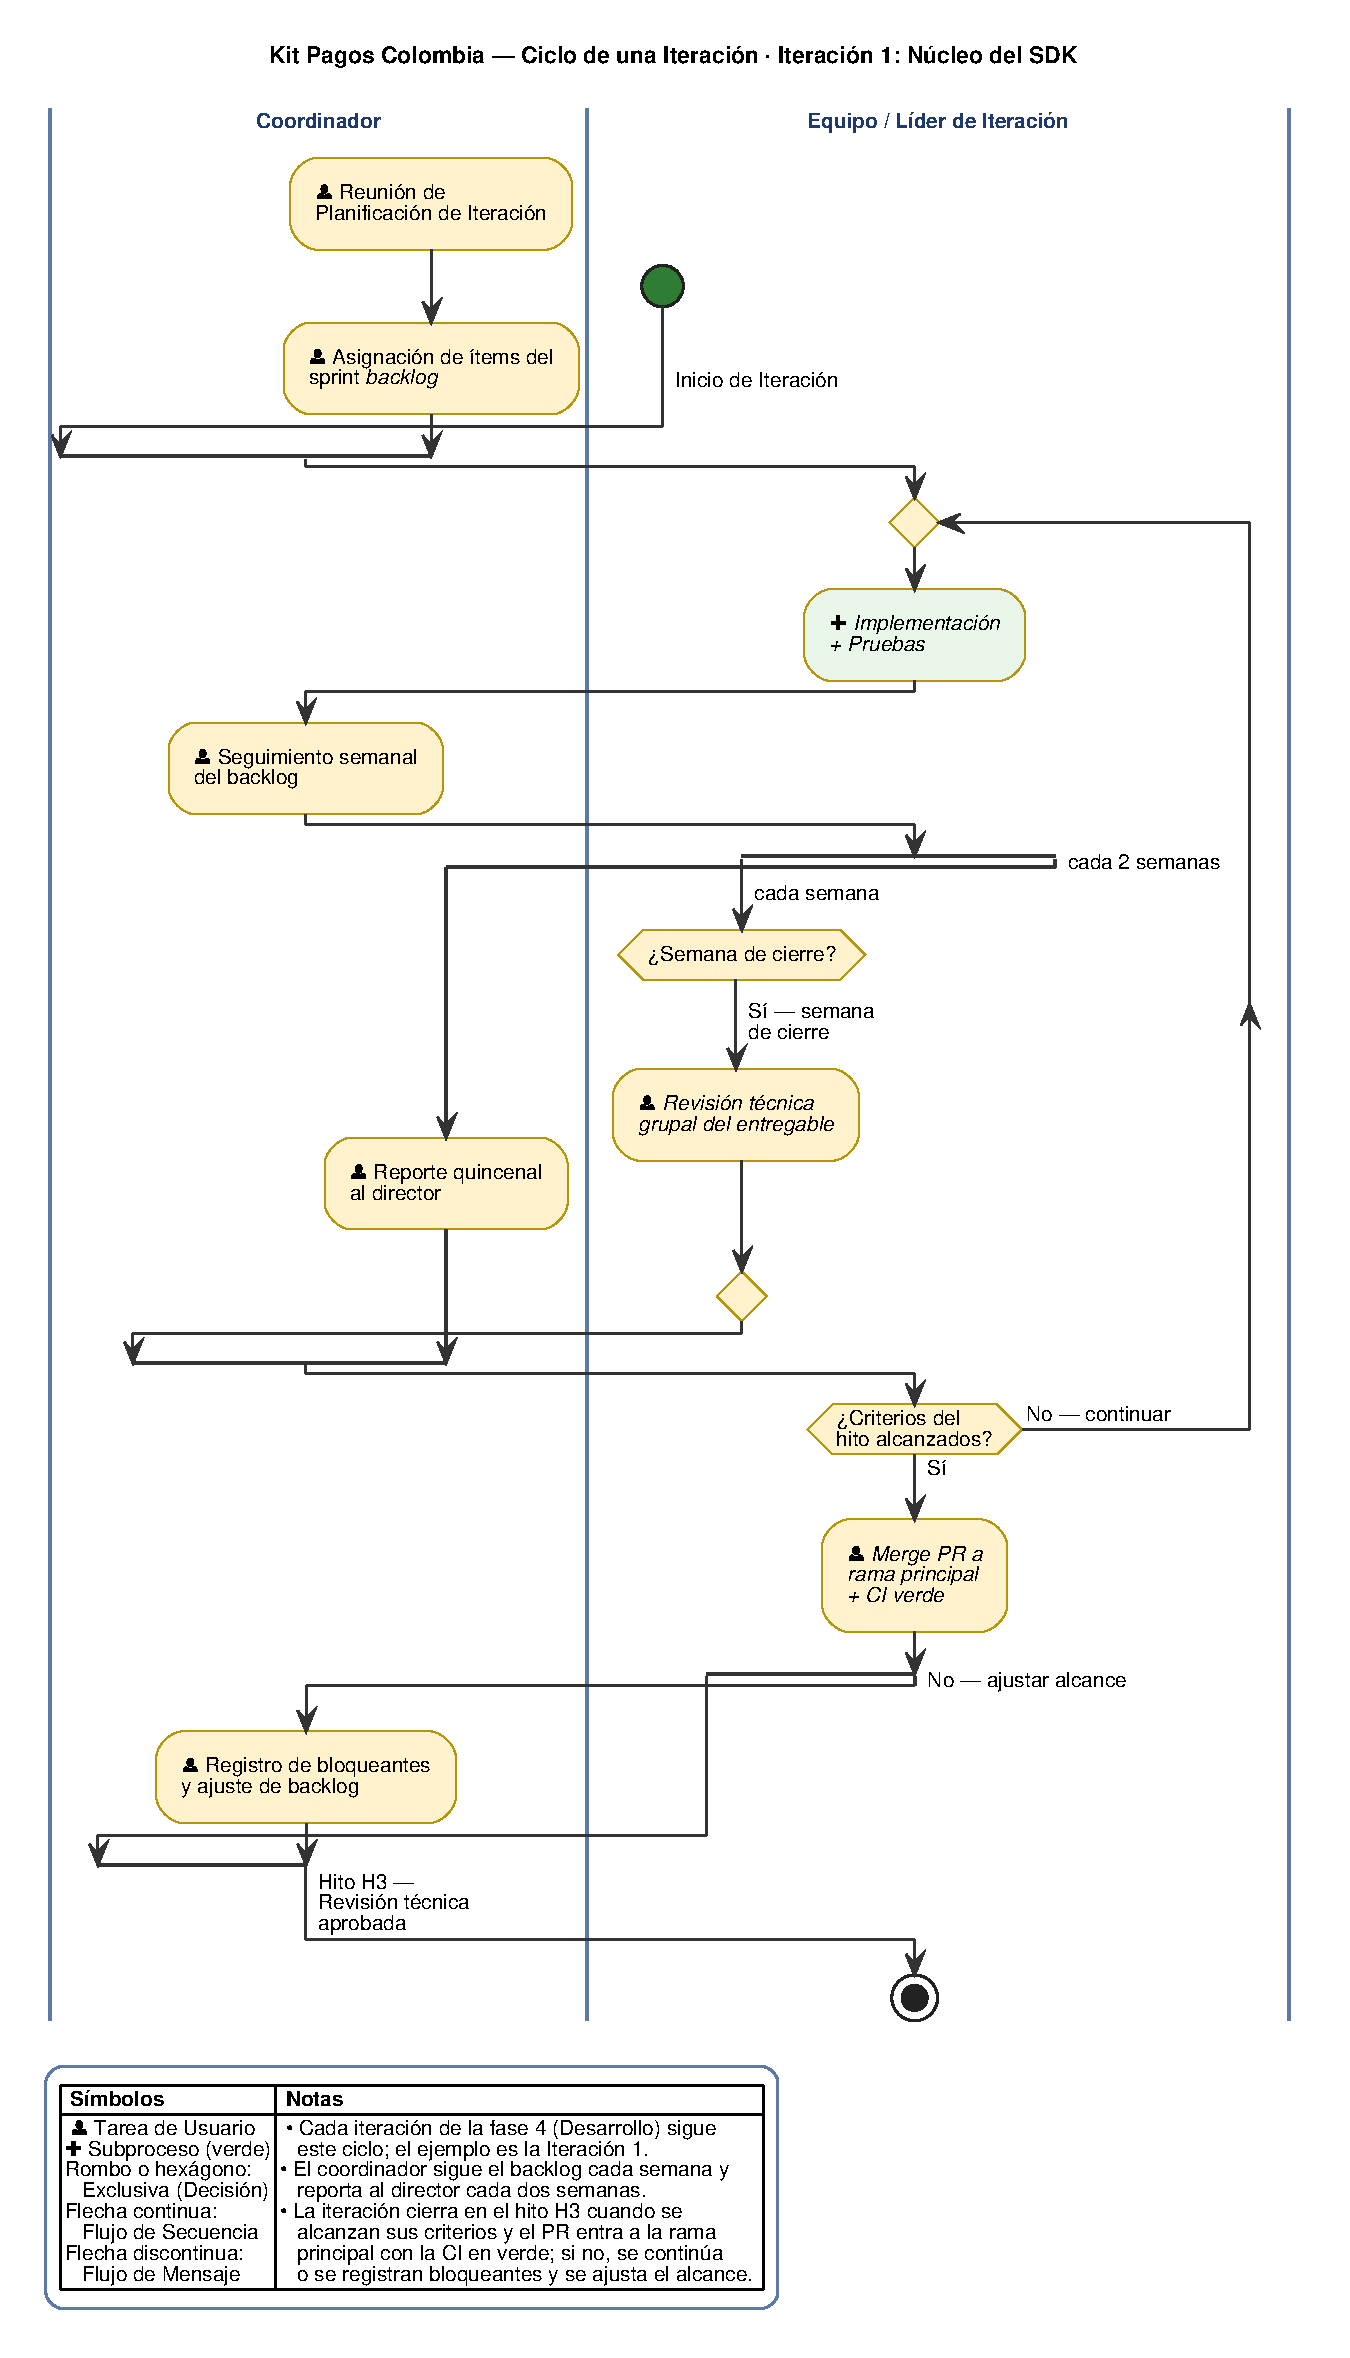
\includegraphics[width=\textwidth]{figuras/04-bpmn-iterativo}
  \caption{Diagrama BPMN iterativo}
  \label{fig:bpmn-iterativo}
\end{figure}

\subsubsection{Asignación de Recursos}

Para cada actividad principal del WBS se indica el conjunto de roles involucrados y las herramientas necesarias para ejecutarla.

\begin{center}
\renewcommand{\arraystretch}{1.2}
\SinNumero
\begin{longtable}{|P{0.213}|P{0.479}|P{0.308}|}
  \hline
  Actividad (WBS) & Roles involucrados & Herramientas \\
  \hline
  \endfirsthead
  \hline
  Actividad (WBS) & Roles involucrados & Herramientas \\
  \hline
  \endhead
  1.1 Gestión del proyecto & Coordinador (primario); todos los integrantes como reportantes & GitHub Projects, Notion, Microsoft Teams, Google Docs \\
  \hline
  1.2 Fase 1 – Identificación & Todos (un integrante por pasarela); Coordinador consolida el mapa del ecosistema & Documentaciones oficiales de las pasarelas, Notion, Draw.io \\
  \hline
  1.3 Fase 2 – Definición & Líder de evaluación redacta el SRS; Coordinador gestiona el backlog; todos revisan y aprueban & Google Docs, GitHub Projects, Notion \\
  \hline
  1.4 Fase 3 – Diseño & Líder de arquitectura lidera; todos revisan los contratos de puerto y los ADRs & Draw.io (UML y BPMN), Notion (ADRs), Google Docs \\
  \hline
  1.5.1 Iter 1 – Núcleo del SDK & Líder de arquitectura (primario); revisión obligatoria de todos antes de iniciar Iter 2 & TypeScript, Jest, GitHub (PR + CI), VS Code \\
  \hline
  1.5.2 Iter 2 – Adaptadores & Líder de integración coordina; cada adaptador se desarrolla en par con otro integrante & TypeScript, Jest, sandboxes de las cuatro pasarelas, GitHub \\
  \hline
  1.5.3 Iter 3 – API de simulación & Líder de integración (primario); Líder de arquitectura apoya en diseño de contratos & Fastify, TypeScript, Railway o Render, Postman, GitHub \\
  \hline
  1.6 Fase 5 – Evaluación & Líder de evaluación lidera; todos construyen los prototipos asignados & ts-morph, TypeScript, Jest, Google Spreadsheets \\
  \hline
  1.7 Fase 6 – Comunicación & Líder de evaluación coordina la redacción del documento; todos contribuyen por secciones; Coordinador gestiona la publicación del repositorio & Google Docs, GitHub, TypeDoc, npm \\
  \hline
\end{longtable}
\end{center}

Los recursos del proyecto son exclusivamente humanos y de herramientas software. No existe hardware dedicado: cada integrante trabaja desde su equipo personal. La disponibilidad de los sandboxes de las pasarelas es un recurso externo no controlado por el equipo; su indisponibilidad prolongada activa el protocolo de riesgo descrito en la sección 7.2.

\subsubsection{Asignación de Presupuesto y Justificación}

Costos reales del proyecto

El proyecto opera íntegramente con herramientas de acceso gratuito. Los únicos costos potencialmente reales son los asociados al despliegue de la API de simulación.

\begin{center}
\renewcommand{\arraystretch}{1.2}
\SinNumero
\begin{longtable}{|P{0.271}|P{0.271}|P{0.12}|P{0.338}|}
  \hline
  Concepto & Período & Costo estimado (COP) & Justificación \\
  \hline
  \endfirsthead
  \hline
  Concepto & Período & Costo estimado (COP) & Justificación \\
  \hline
  \endhead
  Despliegue en Railway o Render & Semanas 10–18 & \$0 & Ambas plataformas ofrecen tier gratuito con recursos suficientes para el volumen de pruebas del proyecto \\
  \hline
  Herramientas de desarrollo (GitHub, npm, TypeScript, Jest, Postman, Notion) & Semanas 1–18 & \$0 & Gratuitas para proyectos open source o uso educativo \\
  \hline
  Dominio y certificado SSL & Semanas 10–18 & \$0 & Las plataformas de despliegue proveen subdominio y HTTPS sin costo adicional \\
  \hline
  Total de costos reales & Semanas 1–18 & \$0 &  \\
  \hline
\end{longtable}
\end{center}

Estimación del costo del software

Aunque no se movilizan recursos financieros reales, el esfuerzo invertido tiene un valor económico equivalente. Para su cálculo se utiliza una tarifa de referencia de COP 25.000 por hora, correspondiente al rango de mercado para un desarrollador junior con competencias en TypeScript y arquitecturas de software en Colombia en 2026.

\begin{center}
\renewcommand{\arraystretch}{1.2}
\SinNumero
\begin{longtable}{|P{0.282}|P{0.282}|P{0.188}|P{0.248}|}
  \hline
  Fase DSR & Período & Horas estimadas & Costo estimado (COP) \\
  \hline
  \endfirsthead
  \hline
  Fase DSR & Período & Horas estimadas & Costo estimado (COP) \\
  \hline
  \endhead
  Identificación del problema & Semanas 1–3 & 87 & 2.175.000 \\
  \hline
  Definición de objetivos & Semanas 3–5 & 69 & 1.725.000 \\
  \hline
  Diseño & Semanas 5–7 & 104 & 2.600.000 \\
  \hline
  Desarrollo iterativo & Semanas 7–13 & 389 & 9.725.000 \\
  \hline
  Demostración y evaluación & Semanas 13–16 & 130 & 3.250.000 \\
  \hline
  Comunicación & Semanas 16–18 & 87 & 2.175.000 \\
  \hline
  Total & Semanas 1–18 & 866 & 21.650.000 \\
  \hline
\end{longtable}
\end{center}

Este cálculo tiene propósito referencial y no implica flujo real de dinero. Su utilidad es dimensionar el valor del trabajo producido y servir como punto de comparación en caso de que proyectos similares requieran contratación externa.
